% Document template based on LNCS, adapted by Matt Welsh <mdw@cs.berkeley.edu> and Mark Hempstead<mhempstead@coe.drexel.edu>

% This version is adapted to use PDFTEX to render to PDF directly. 
% If you want to use dvi, you need to change any figures to use '.eps'
% rather than '.pdf', and probably get rid of the hyperref package.

\documentclass{article}
\usepackage{program}
\usepackage{acm-style10} % ACM proceedings formatting
\usepackage{times}       % Use Adobe Times font set
\usepackage{epsfig,twocolumn}
\usepackage{url}
\usepackage[english]{babel} % mdw: Required to get good hyphenation on RH6.0
                            % (fixed in RH6.1)
\usepackage{graphicx} 
\usepackage{color}

% DO NOT EDIT THE BELOW BLOCK OF CODE
\def\dsp{\def\baselinestretch{1.10}}
\dsp
\newcommand{\XXXnote}[1]{{\bf\color{red} XXX: #1}}
\setlength{\textheight}{9.25in}
\setlength{\columnsep}{0.33in}
\setlength{\textwidth}{7.4in}
\setlength{\footskip}{0.0in}
\setlength{\topmargin}{-0.25in}
\setlength{\headheight}{0.0in}
\setlength{\headsep}{0.0in}
\setlength{\oddsidemargin}{-.45in}
\setlength{\parindent}{1pc}
\pagestyle{empty}
\begin{document}
\date{}

%%%%%%%%%%%% THIS IS WHERE WE PUT IN THE TITLE AND AUTHORS %%%%%%%%%%%%

% Title here
\title{\ttlfnt My EE 194 Project Paper}

% Author names, affiliations, and e-mail below
\author{{\aufnt Mark Hempstead} \\ 
{\affaddr Tufts University} \\ 
{\affaddr mark.hempstead@tufts.edu}}

\maketitle
%\copyrightspace
\thispagestyle{empty}

%%%%%%%%%%%%%  ABSTRACT GOES HERE %%%%%%%%%%%%%%

\subsection*{Abstract}
\begin{small}
This is a template for a paper for Advanced Computer Architecture using PDFLaTeX.
This is supposed to be the abstract, but as you can see, it doesn't
have a lot of content. In the abstract you should summerize the problem, your approach, and results. I have created a makefile for you, simply type \texttt{make} at the terminal to compile.
\end{small}

%%%%%%%%%%%%%  BODY OF PAPER GOES HERE %%%%%%%%%%%%%%

% Generally you will want to break the paper into separate sections
% and use \input{...} to include them, like so:
%\input{intro.tex} 
%\input{motivation.tex}
%\input{design.tex}
%\section{Implementation Details}\label{sec:implementation}

Gradient descent entropy minimization is an instance of a ``matric-based''
algorithm. Metric-based autofocus algorithms accept a complex image represented
as an array of pulse contributions and obtain a phase offset vector which, when
applied to the original pulses, optimizes a given metric. We can express this
precisely by considering that in backprojection each radar pulse, $\vec{b_i}$,
contributes information to each pixel, $z_i$, to form a final image. To model
this, let each $\vec{b_i}$ be a matrix whose value at some point $(x,y)$
corresponds to the contribution of pulse $i$ to the pixel at $(x,y)$.  For $K$
pulses we have the pulse set $\{\vec{b}_1, \vec{b}_2, \dots \vec{b}_K\}$,
the sum of which forms the image matrix $\zb$.

Consider an image of $N$ pixels. Each pixel can be computed as:

\begin{equation}\label{eq:complex_image}
z_n = \sum_{i=1}^{K} b_{i,n}
\end{equation}

where $b_{i,n}$ is the $n$-th pixel for pulse $i$. As discussed, SAR data are
plagued by phase errors which can be modeled as per-pulse phase shifts:
$\phib = \{\phi_1, \phi_2, \dots \phi_k\}$. Applying this to
Eq.~\ref{eq:complex_image} yields:

\begin{equation}\label{eq:phase_complex_image}
z_n = \sum_{i=1}^{k} b_{i,n}e^{-j\phi_i}
\end{equation}

The goal of gradient descent autofocus is to optimize over a image quality
metric. We use image entropy, defined as~\cite{kragh2006monotonic}:

\begin{equation}\label{eq:entropy}
  H(\zb) = \sum_{n=1}^{N} \frac{|z_n|^2}{E_z} \ln
  \frac{|z_n|^2}{E_z}
  \text{,\indent} E(\zb) = \sum_{n=1}^{N} |z_n|^2.
\end{equation}

In Eq.~\ref{eq:entropy}, $\zb$ is a complex image, and $E_z$ is
the total image energy. We therefore seek:

\begin{equation}\label{eq:arg_min}
  \vec{\hat{\phi}} = \argmin(H(\zb(\phib)))
\end{equation}

Eq.~\ref{eq:arg_min} has no closed form solution~\cite{ash2012autofocus}. As
mentioned we employ gradient descent optimization. That is, we minimize the
objective function, $H$, first by forming an approximation to its gradient,
$\nabla H$. Next, we iterate down the negation of the gradient to find a
minimum. Therefore, the $l$-th iteration can be expressed as:

\begin{equation}\label{eq:recursion}
  \phib^l = \phib^{l-1} - s \nabla H(\zb(\phib^{l-1}))
\end{equation}

where $s$ is a scalar step size and the gradient of $H$ is with respect to
$\phib$. Eq.~\ref{eq:recursion} is evaluated by approximating the gradient
$\gb \equiv \nabla H(\phib^{l})$ via the following algorithm:

\begin{algorithm}
  \caption{Finite difference approximation of $\gb$}
  \label{alg:finitediff}
  Let $\eb_i$ be the $i$-th column of a $K \times K$ identity matrix.\\
  Let $\delta$ be some small offset.\\
  \ \\
  $H_0 \gets H(\zb(\phib^l))$\\
  \ \\
  \For{$i = 1,2,\dots, K$}{
    $H_i \gets H(\phib^l+\delta \times \eb_i)$\\
    $g_i \gets (H_i - H_0)/\delta$\\
  }
  \ \\
  \Return $\gb$
  \vspace{5 mm}
\end{algorithm}

The above computes the finite difference approximation to the gradient. By
iterating this recursive formulation until the image entropy converges, the
complex image can be computed via Eq.~\ref{eq:phase_complex_image} to yield a
focused image.

We exploit the data parallelism inherent in Alg.~\ref{alg:finitediff} in both
our reference MATLAB as well as C++ and CUDA implementations. Transitioning to a
C++ based solution offers much more efficient and finegrained thread control and
reduced memory footprint. Also, the performance difference between C++ and
MATLAB is well known. The next two subsections discuss the optimizations we
employed to improve performance and reduce complexity. 
 
\subsection{Reusing $\zb_{0}$}

The primary optimization we developed came from the ``reuse'' of the image
computed for $H_0$ in the first step of Alg.~\ref{alg:finitediff}. As shown by
Eq.~\ref{eq:phase_complex_image} and~\ref{eq:entropy}, computing $H_0$ requires
$\zb(\phib^l)$ as an intermediary value. In principle, this intermediary is
distinct for each $H_k$, but can be expressed by a function of $\phib^l$ and
$\delta$. That is, for each iteration of Alg.~\ref{alg:finitediff}, a given
$\phi_{i}$ is offset by $\delta$.  Substituting into
Eq.~\ref{eq:phase_complex_image} yields $z'_n$:

\begin{equation}\label{eq:z_prime}
  \begin{split}
    z'_n = z_n + b_{i,n}e^{-j(\phi_{i} + \delta)} - b_{i,n}e^{-j\phi_{i}} \\ =
    z_n + b_{i,n}e^{-j\phi_{i}}(e^{-j\delta} - 1)
  \end{split}
\end{equation}

Let $\alpha_{i} = e^{-j\phi_{i}}(e^{-j\delta} - 1)$. Thus, for each $H_i$, we
can express $\zb_{i} = \zb_{0} + \alpha_{i} \vec{b}_i$. Without this
optimization, Alg.~\ref{alg:finitediff} took $K$ iterations, each of which
summed over $N$ pixels, each requiring $K$ operations to evaluate, for a bound
of $\Theta(NK^2)$. Using this technique, a given pixel $z_i$ can be computed in
constant time after $H_0$ has been computed. This reduces to only $N$ operations
per iteration of Alg.~\ref{alg:finitediff} for $NK$ operations plus an
additional $NK$ operations to compute $H_0$, resulting in a complexity of only
$\Theta(NK)$.

\subsection{Reducing Memory Constraints}

Additionally, the expression for $H$ can be implemented more efficiently as:

\begin{equation}\label{eq:eff_entropy}
  H(\zb) = \frac{1}{E_z}(\sum_{n=1}^{N} |z_n|^2 \ln |z_n|^2 - E_z \ln E_z)
\end{equation}

In this form, Eq.~\ref{eq:eff_entropy} can be computed incrementally, building the
two summations concurrently as $\zb$ is evaluated. This allows the input phase
history to be partitioned at an arbitrary number of pixels, $N' \le N$, to match
the memory constraints of the system. We can, therefore, accumulate the summation
term and $E_z$ as each partition is processed. This was critical for the tight memory
limits of the GPU when image sizes exceeded the 2 GB of main memory. As
discussed in~\cite{gpu-sar} and shown by our results in
Section~\ref{sec:results}, the overhead of these data transfers can reduce
performance and so reducing the size of required temporary arrays alleviates
this issue.

%\input{evaluation.tex}
%\input{conclusion.tex}

\section{Introduction}

Some text for the introduction would go here.
It is important that your paper be well-written, as if you were to
submit it to a conference. 

The first sentence of each paragraph should summarize what the
paragraph is about. I usually write by sketching the outline of the
paper and then writing one or two poorly-formed sentences that capture
what each paragraph is going to say. Then I go through the paper and
rewrite each paragraph, one at a time, until it sounds right.
The sketch document is very useful for helping you see where you are
going next, and organizing your thoughts before crafting the actual
sentences.


Here is an example of how to cite various papers, books, and so
forth~\cite{nesc-pldi03,shewchuk-delaunay}.


\section{Project Description}

Use a section or two to describe your project motivation, goals, research approach or proposed solution to the problem. The Section headings should be appropriate for the material dicussed by the paper. Think of some of the section headings in the papers we read. For example:
\begin{itemize}

\item \textbf{Transactional Memory } this was Section 2 in the Transactional Memory Paper. Using a heading like this conveyed to the reader that this is a new, and important concept.

\item \textbf{Telsa Archiecture} in the \textit{Telsa} paper this section provided the overview of the architecture. \small{(Notice how I'm showing you how to change font styles in \LaTeX{}.)}

\end{itemize} 

\subsection{Specific Detail}

Subsections are very useful for providing structure and making it easy for the reader to follow your dense material. Think about some of the example You might want to include a figure or diagram describing the system, project, or approach.


\section{Experimental Methodology}

Use this section to describe all of the details of your equipment, simulator, CAD tools, or compiler. This is where you list the versions of the tools you used and the configurations. For architecture simulations I recommend including a table with all of the architecture configurations. Then refer the table: Table~\ref{tab:cpu_configs} describes the different architecture parameters that we tested, this is a very complicated table using multicolumn to merge certain collums. For a simple example see Table~\ref{tab:bm} in Section~\ref{sec:results} that provides a summary of our results by benchmark.

\begin{table}[t]
  \begin{center}
      \small{
          \begin{tabular}{ |r||c|c|c| }
          \hline
          \multicolumn{4}{|c|}{2-way Bobcat} \\ \hline
          Item & Baseline OoO & BOLT & SCREW \\ \hline \hline 
          Clock & \multicolumn{3}{c|}{1600 MHz} \\ \hline  
          BPred & \multicolumn{3}{c|}{3-table PPM: 256$\times$2, 128$\times$4, 128$\times$4}\\ 
                & \multicolumn{3}{c|}{8b tags, 2b counters} \\ \hline \hline
          IQ & \multicolumn{3}{c|}{24 entries} \\ \hline
          Regfile &\multicolumn{3}{c|}{120 pregs (64 arch + 56 rename)} \\ \hline
          ROB  &  \multicolumn{3}{c|}{56 entries} \\ \hline
          \hline
          L1 I\$& \multicolumn{3}{c|}{32KB, 256-set, 2-way, 64B blocks, 3-cycles} \\ \hline
          L1 D\$ & \multicolumn{3}{c|}{32KB, 64-set, 8-way, 64B blocks, 3-cycles} \\ \hline
          L2 \$ &\multicolumn{3}{c|}{512KB, 512-set, 16-way, 64B blocks, 16-cycles} \\ \hline
          Mem &\multicolumn{3}{c|}{tCAS: 10ns, tRAS:45ns, tRP:15ns} \\ \hline
          \hline
          Slice Buffer & --- & 64 & 64 \\ \hline
          Chkpoints  &--- & 2 & 2 \\ \hline
          \hline
          SQ type & SQIP & SQIP/CSB & SQIP/CSB \\ \hline
          SQ size & 22 & 64 & 64 \\ \hline
          LQ type & SVW & SVW & SVW \\ \hline
          LQ size & 24 & 96 & 96 \\ \hline
      \end{tabular}
          \vspace{12pt}
      \caption{\textbf{Simulated processor configurations.} This table describes the three different processor configurations we studied. For example the cache, and branch predictors are the same, but the size of the load and store queues are different.}
      \label{tab:cpu_configs}
  }
  \end{center}
\end{table}  



\section{Results and Analysis}
\label{sec:results}  %labels are useful if you want to be able to refer to sections in other places in the text.

In this section you should describe your results and analyze the data. Do not just point to the figure. Explain the data and tell the reader something interesting about the results. If you can say anything interesting then show another figure.

Here is an example of how to include a figure 
(see Figure~\ref{fig-knearest-perf}). You can use PDF, JPEG, 
or PNG files as figures. If you have a PostScript or EPS file, use
{\tt epstopdf} to convert it to PDF first. Generally it is a bad idea
to use bitmap graphics, since they don't look good on screen or in
print. 

% Use 't' to put the figure at the top of the page. This is going to
% look a little strange on the one-page template file, but works fine
% with a multi-page paper.
% The 0.8\hsize directive makes a figure that is 80% of the collumn width.
%
% Note if you need your figure to span both collumns use \begin{figure*} and \end{figure*} instead.
\begin{figure}[t]
\begin{center}
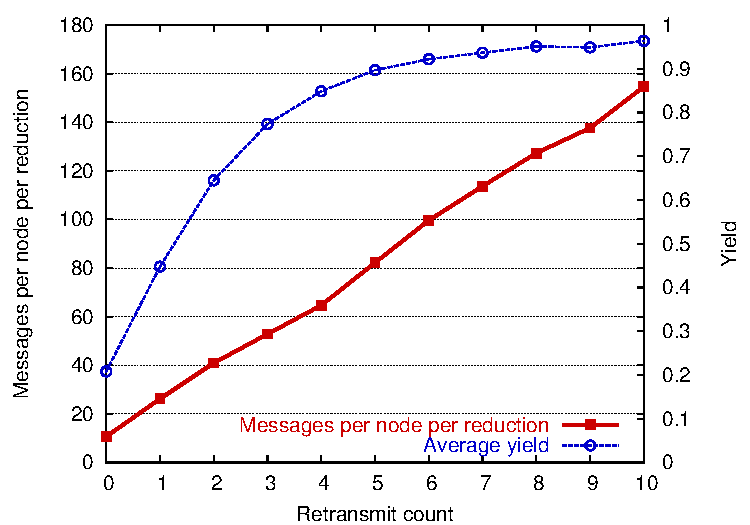
\includegraphics[width=0.8\hsize]{./figures/reduce.pdf}
\end{center}
\caption{{\small {\bf Reduction yield and overhead in the 
$k$-nearest neighborhood region.} {\em This figure shows the average 
yield (fraction of neighbors responding to a reduction request) and
number of messages for reduction operations. The yield and overhead 
are directly related to the number of retransmission attempts made by 
the transport layer.}}}
\label{fig-knearest-perf}
\end{figure}


\begin{table}[h]  %places the table ``here''
    {    \small
\begin{tabular}{|l|l|l|l|l|l|l|l|l|}
\hline
Bmk & IPC &L2 MLP & L2 MPKI & L3 MLP & L3 MPKI \\ \hline  \hline 
\bf cactusADM & 1.07 & 4.10 & 4.73 & 4.42 & 2.75 \\ \hline 
calculix & 1.53 & 1.94 & 2.18 & 3.75 & 0.52 \\ \hline 
dealII &  1.62 & 1.83 & 2.66 & 3.52 & 0.30 \\ \hline 
gamess &  1.68 & 1.42 & 1.63 & 2.47 & 0.10 \\ \hline 
\bf GemsFDTD & 1.08 & 2.42 & 10.09 & 4.04 & 3.00 \\ \hline 
\bf lbm & 0.59 & 4.99 & 38.81 & 4.39 & 18.13 \\ \hline 
\bf milc & 0.50 & 2.46 & 24.44 & 2.74 & 14.64 \\ \hline 
namd & 1.55 & 1.73 & 0.14 & 2.91 & 0.03 \\ \hline 
povray & 1.38 & 1.55 & 0.06 & 2.86 & 0.00 \\ \hline 
\bf soplex & 0.59 & 2.21 & 24.27 & 2.91 & 8.23 \\ \hline 
\bf sphinx3 & 1.27 & 2.02 & 14.16 & 3.46 & 1.17 \\ \hline 
tonto & 1.66 & 1.43 & 0.20 & 2.14 & 0.03 \\ \hline 
wrf & 1.44 & 2.16 & 5.81 & 4.33 & 0.48 \\ \hline 
\bf zeus & 1.00 & 1.98 & 6.83 & 3.59 & 2.69 \\ \hline 
\hline
astar & 0.83 & 2.01 & 5.29 & 2.20 & 0.05 \\ \hline 
bzip2 & 1.44 & 2.31 & 3.28 & 2.52 & 0.08 \\ \hline 
gcc & 1.21 & 1.39 & 3.37 & 1.90 & 0.49 \\ \hline 
gobmk & 0.98& 1.50 & 2.03 & 1.65 & 0.20 \\ \hline 
h264ref & 1.90 & 1.43 & 1.76 & 1.66 & 0.05 \\ \hline 
hmmer & 1.36 & 1.36 & 0.00 & 2.45 & 0.00 \\ \hline 
\bf libquantum & 98.7 & 3.01 & 21.96 & 3.53 & 0.00 \\ \hline 
\bf mcf & 0.21 & 2.53 & 112.37 & 2.35 & 17.62 \\ \hline 
omnetpp & 1.22 & 1.26 & 0.17 & 1.48 & 0.12 \\ \hline 
sjeng & 0.96 & 2.96 & 7.71 & 7.67 & 1.40 \\ \hline 
xalancbmk & 1.22 & 1.62 & 2.62 & 2.99 & 0.14 \\ \hline 
\end{tabular}
}
\vspace{10pt} %sometimes you need to force spacing, depends on the template file.
\caption{\textbf{SPEC2006 Benchmarks Data} Includes data for IPC, and cache miss rate.}
\label{tab:bm}
\end{table}

Sometimes it is better to show data with a table. Table~\ref{tab:bm} provides an example. Notice here we have included all of the miss rates and then bolded the benchmarks that we found interesting and that we are going to explain in the text.



\section{Conclusion}

In this section you should summerize the problem and your results. The conclusion section often contains a paragraph at the end that describes future work and leaves the reader with a good impression of the papers contributions. \textit{Real researchers use \LaTeX{}!}


%%%%%%%%%%%%%  THIS IS WHERE THE BIBLIOGRAPHY GOES %%%%%%%%%

% Change the word "template" below to the name of the .bib file you use
\begin{small}
\bibliographystyle{abbrv} \bibliography{template}
\end{small}

\end{document}

